\chapter{Gait Watch and Qualisys Optica motion tracker}
\label{ch:GWandQS}

\section{Introduction and chapter's structure}
After explaining and comparing both systems Gait Watch and Force Plate, we proceed now to do analysis of te differences and similarities between Gait Watch and Qualisys Optical motion tracker.

It has been demonstrated that Qualisys System is a accurate system to analyse the body movements and it can be used in several applications. However, this system has a lot of constraints like the possibility of application scope.

Thus, we are going to do a comparison with Gait Watch system, a system based in inertial sensors being more potable and cheaper.
Along this chapter we will explain how the pitch has been calculated using Qualisys System. This will be what we will compare with the angles obtained through inertial sensors.


\section{Computing Euler angles using Qualisys System}
To compute the Euler angle, the subject is wearing two infrared markers per segment placed in both thighs and shanks. The infrared optical cameras emit infrared light and this reflects in the markers placed over the body allowing to know the position of the markers.

The pitch angle of such segment is computed between the vector defined by the upper and lower markers and the vector normal to the Earth’s surface. To be able to compute it we first have to define a third point which has the same X coordinate as the lower marker and the same Z coordinate as the upper marker. This will define a right triangle in which one of the contiguous cathetus is normal to the Earth’s surface and the hypotenuse is defined by the line between the upper and the lower point. Therefore, by calculating the arctangent we can easily find the angle of the right triangle, which is, in turn, the pitch angle\cite{OlivaresBotzel2013}. We can see this in \ref{fig:pitchQS}

\begin{figure}[H]
	\centering
	\epsfig{file=imagenes/pitchQS, width=7cm}
	\caption{Diagram of the pitch computation using the Qualisys System \cite{OlivaresBotzel2013}.}
	\label{fig:pitchQS}
\end{figure}

Thus, the pitch angle is computed as follows:

\begin{equation}
\label{angleQS1}
	\theta_{QS}= arctang(\frac{a}{b})
\end{equation}

\begin{equation}
\label{angleQS2}
	a= \sqrt{(x_{upper}-x_{lower})^{2} + (z_{upper}-z_{upper})^{2} }
\end{equation}

\begin{equation}
\label{angleQS3}
	b= \sqrt{(x_{lower}-x_{lower})^{2} + (z_{lower}-z_{upper})^{2} }
\end{equation}

where $ [x_{lower}, z_{lower} ] $ and $ [x_{upper}, z_{upper} ] $ are the coordinates of the projections of the lower an upper markers in the XZ plane, respectively.

\section{Feature extraction}
In this experiment, prior to start of data gathering, we set up the protocol for procedure that people have to carry out while the data are recorded. Seven control subject have been involved. They had to walk during some minutes over a treadmill with differents speeds, specifically 2, 4 and 6 Km/h.

This movements is characterised by the Gait Watch system and Qualisys System. To do this, the participants wear the inertial sensors over the body and the infrared markers, being these last one visibles by infrared cameras all the time. This experiment is carried out in a control environment where both systems can work properly.

One the data have been gathered, we proceed to do a signal processing before the features extraction. For the GW signals, the procedure is the same than in above cases. The first step is doing the calibration and correct the erroneous values in the signals due to a noise of the sensors.
Then, we can figure out the angle of the differents segments of the body. The program done in Matlab allows us choose what segments we can use to calculate and compare between both systems. In this case, we can select: right shank, left shank, right thigh and left thigh.

The angle of these segments are calculated for each point of time with a sample frequency of 200 samples/s for both systems so we don’t have to interpolate because these signals match perfectly. The pitch is filtered with a Kalman Filter in the GW signals because it is an algorithm that uses measurements observed over the time and produces estimates of unknown variables that tend to be more precise than others base on a single measurement. In other words, Kalman Filter operates recursively on stream of noisy inputs data to produce a statistically optimal state of the underlying system state\cite{KalmanFilter}.

Hereafter, we calculate the pitch using the QS signals. To to this, we will apply the equations described in the prior chapter \ref{angleQS1}.
After this, we have to center all of these signals and we will be ready to compare all signals now.

\begin{figure}[H]
	\centering
	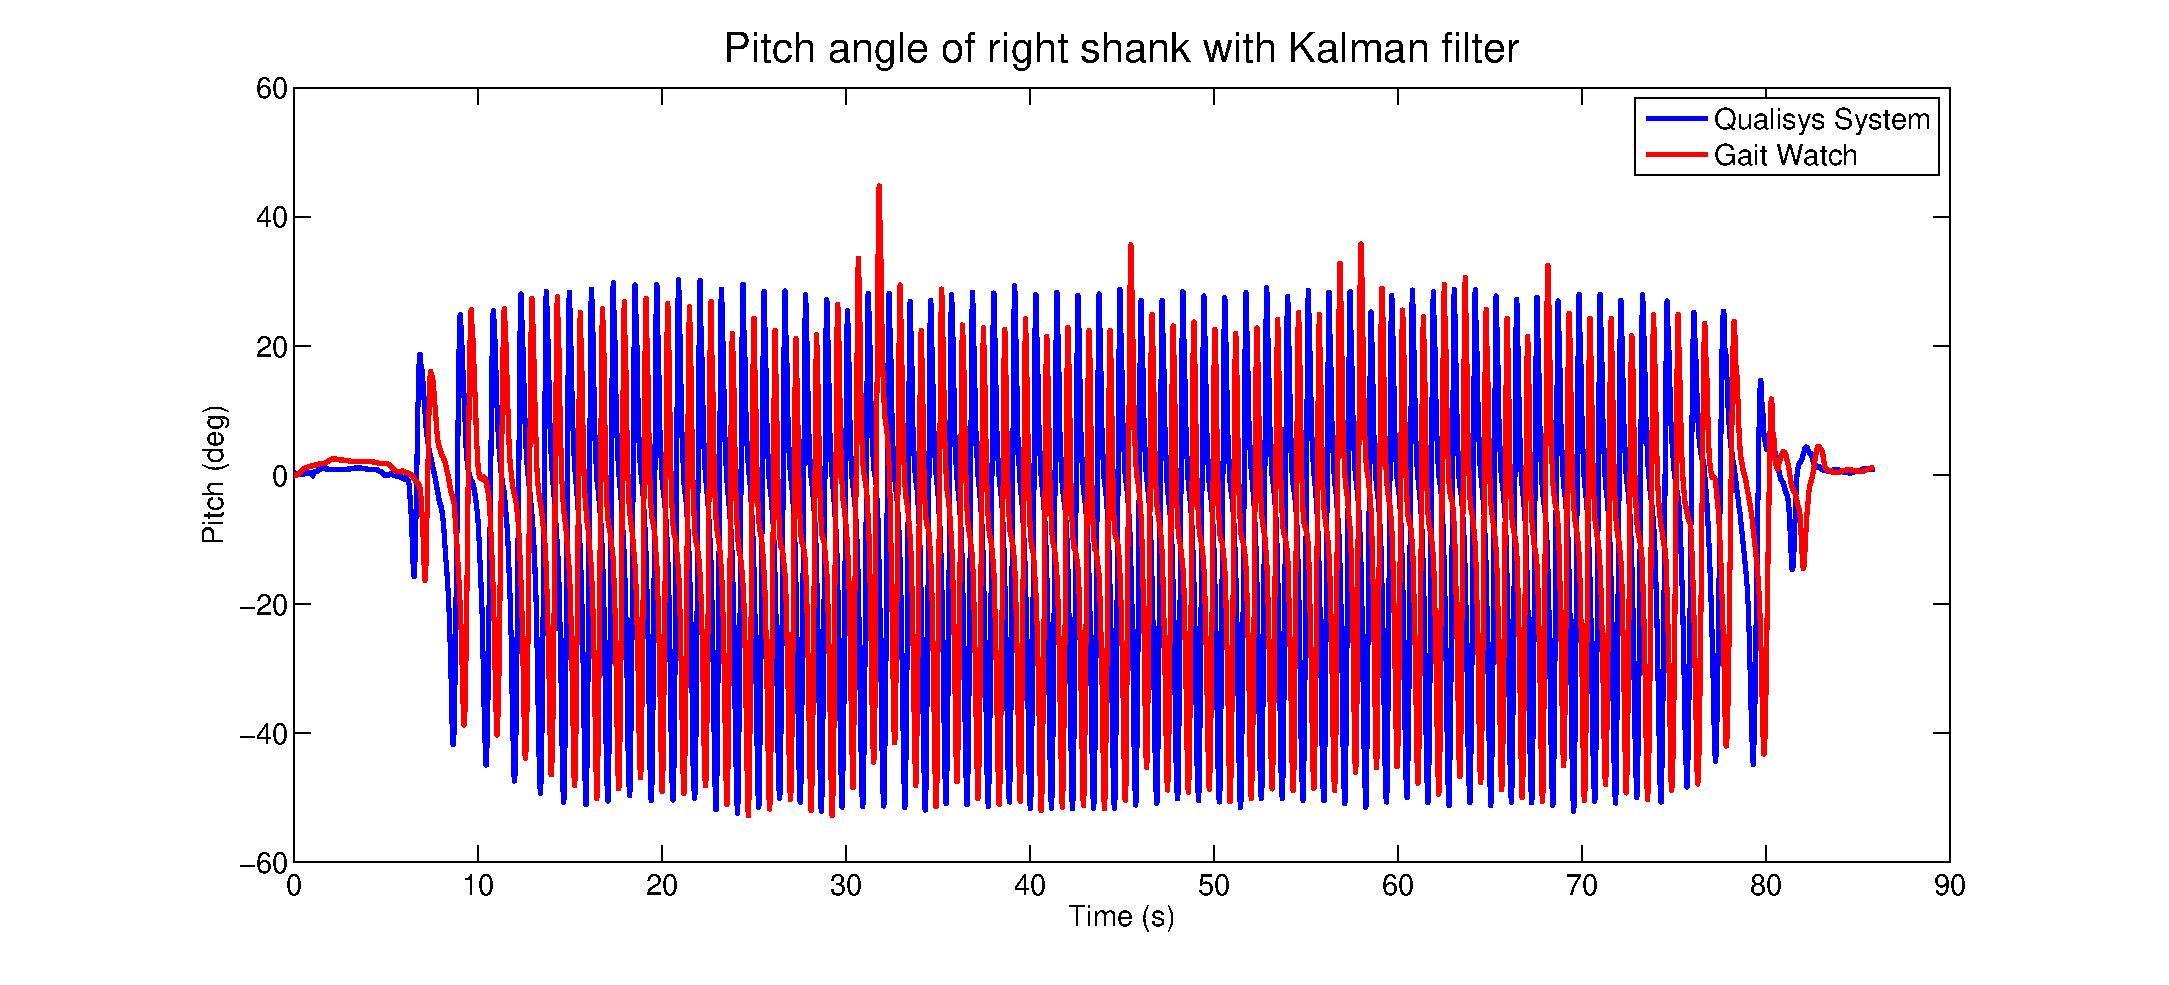
\epsfig{file=figures/QSvsGW/signalGWQS, width=18cm}
	\caption{Pitch angle of right shank for 4Km/h of speed.}
	\label{fig:signalGWQS}
\end{figure}

The next step is the feature extraction. We have to differentiate two comparison. Firstly, we are going to compare the pitch calculated with inertial sensors (GW) and infrared cameras (QS), so we will extract some specific characteristics to do this. After, we are going to compare the angle obtained in function of the speed.

The first feature computed was the ‘stride time’ \ref{fig:featuresGWQS}. This is the time that a person needs to carry out a step, i.e the time since the foot is lifted from the treadmill until the moment when the same foot touches the ground and gains momentum to step again. In the pitch signal, we determine this detecting the distance between two negative value of the pitch because the negative values happen when the segment (shank or thigh) are behind the trunk , this is just before stepping.

Other important aspect is the difference of angle obtained in both systems. We calculate values positives as well as negatives and finally obtain the mean of the difference of all them \ref{fig:featuresGWQS}.
\begin{figure}[H]
	\centering
	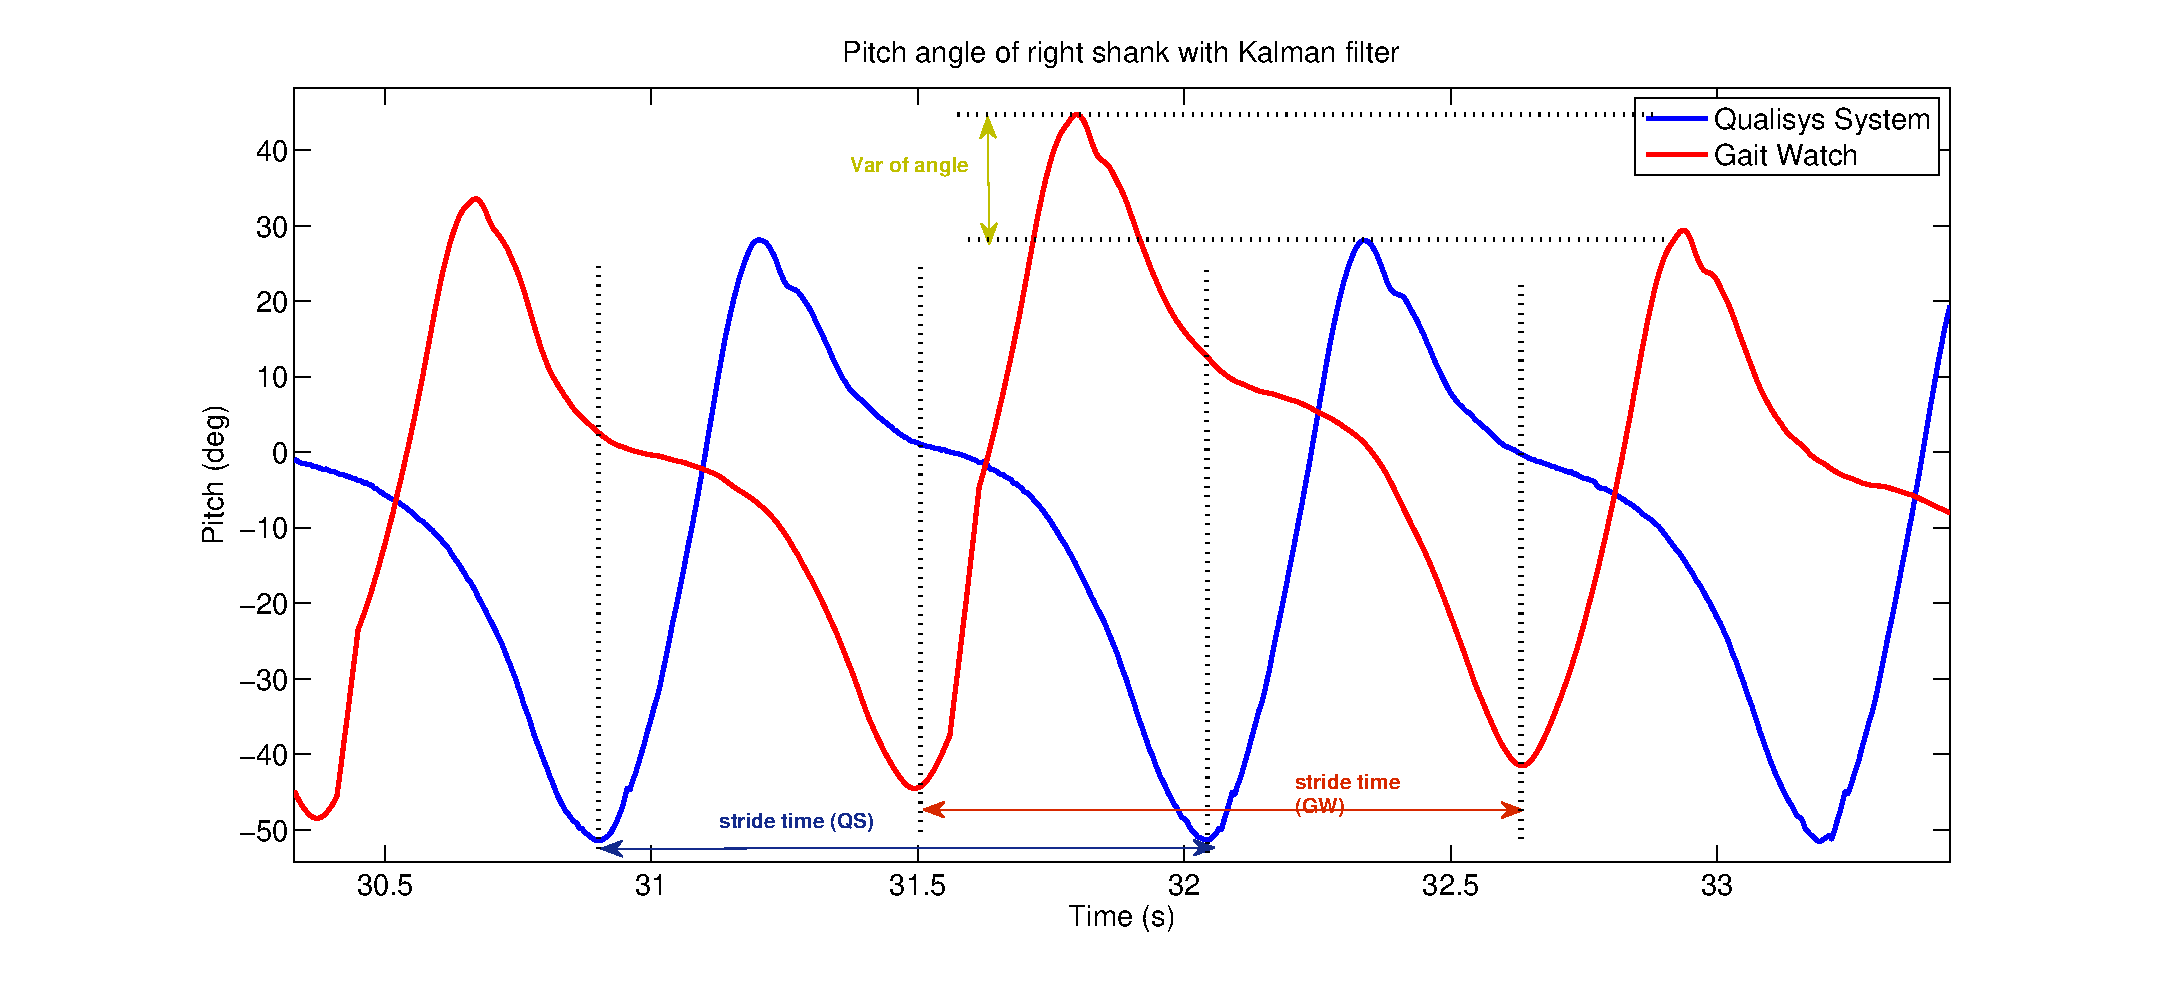
\epsfig{file=figures/QSvsGW/features_GWQS, width=18cm}
	\caption{Features for pitch angle in GW and QS signals.}
	\label{fig:featuresGWQS}
\end{figure}

\section{Results discurssion}

